
	\documentclass{article}
	\usepackage{amsmath,amssymb}
	\usepackage[inline]{enumitem}
	\usepackage{blindtext}
	\usepackage{booktabs}
	\usepackage{graphicx}
	\usepackage{xcolor}
	\usepackage[vmargin = 1.5in, top = 1in, bottom = 1.2in, letterpaper]{geometry}
	\usepackage{listings}
	\usepackage{courier}
	\usepackage{multicol}
	\usepackage{multirow}
	\usepackage{bm}
	\lstset{
	basicstyle = \small\tt,
	keywordstyle = \tt\color{blue},
	commentstyle = \it\color[cmyk]{1,0,1,0},
	stringstyle = \tt\color[RGB]{128,0,0},
	%frame = single,
	backgroundcolor = \color[RGB]{245,245,244},
	breaklines,
	extendedchars = false,
	xleftmargin = 2em,
	xrightmargin = 2em,
	aboveskip = 1em,
	tabsize = 4,
	showspaces = false
	}
	\begin{document}
	
	% \newfontfamily\courier{Courier New}

	
	\title{STAT 601 Homework 1}
	\author{Yifan Zhu}
	\maketitle
	
	\begin{enumerate}[leftmargin = 0 em, label = \arabic*., font = \bfseries]
	\item 
	For series 1 data, to test the model with estimated link against model with fixed logit link, we first fit the model with fixed logit link and by R function \verb|basicglm| from STAT 520 obtained the fited parameters $\hat{\bm \beta}_{basic, 1} = (-60.53546, 14.84114)$ and log likelihood $\ell_{basic, 1} = -89.93966$. Then a model with estimated link is fitted. The parameterized link function is as below
	\[g(\mu | \lambda) = \log\left[\frac{(1 - \mu)^{- \lambda} - 1}{\lambda}\right]\]
	Parameters are estimated by maximizing log likelihhod function. Fisher scoring algorithm is used to maximize log likelihood and R code was written following page 8 - 11 in course notes. The starting values for series 1 data were taken to be result from basic glm and $\lambda$ being 1, which is (-60.53546, 14.84114, 1). With this starting point, the algorithm converges and estimated parameters are $\hat{\bm \beta}_{para, 1} = (-41.567144, 10.074929), \hat{\lambda}_1 = 0.114924$, and log likelihood is $\ell_{para, 1} = -88.66651$. Then the LRT statistic is
	\[-2 (\ell_{basic, 1} - \ell_{para,1}) = 2.5463\]
    Degrees of freedom is the $\chi^2$ distribution here is 1, so p-value is 0.1105529. With p-value greater than 0.05, we fail to reject the null hypothesis and conclude that logit link is good here.

    For series 2 data, we repeat the same procedure. But to make the algorithm converge, results from series 1 data was used to be the starting value. Finally we have two log likelihoods from basic glm and glm with parameterized link, $\ell_{basic, 2} = -95.58295, \ell_{para, 2} = -93.46301$. Then LRT statistic for series 2 data is
    \[-2 (\ell_{basic, 2} - \ell_{para,2}) = 4.23988\]
    Degrees of freedom is the $\chi^2$ distribution here is 1, so p-value is 0.03948496. With p-value less than 0.05, we reject the null hypothesis and conclude that logit link is not good here.


    \item 
    We use LRT to determine whether there is difference between the two serieses. We have fitted series 1 and series 2 to glm with parameterized link and obtained log likelihoods $\ell_{para, 1}$ and $\ell_{para, 2}$. Now we combine two serieses and also fit the combined data to glm with parameterized link. The log likelihood is then $\ell_{para, 12} = -182.3335$. Then the LRT statistic is
    \[-2 (\ell_{para, 12} - \ell_{para, 1} - \ell_{para, 2}) = 0.40796\]
      Degrees of freedom is the $\chi^2$ distribution here is 3, so p-value is 0.9385933. With a big p-value greater than 0.05, we fail to reject the null hypothesis and conclude that there is no significant evidence that there is difference between the two series.


      \item 
      From 3 we see no difference in these two series, so we decide to use one glm with parameterized link for both series. The fitted parameters are $(\hat{\beta}_0, \hat{\beta}_1, \hat{\lambda}) = (-39.71489061, 9.60945493, 0.01221563)$. With estimated parameters, the response curve is
      \[\hat{y}_i(d_i) = G(d_i) = 1 - \frac{1}{(1 + \hat{\lambda} \exp(\hat{\beta}_0 + \hat{\beta}_1 \log d_i))^{1/\hat{\lambda}}}\]
      Since $G$ is cdf of dose, then pdf is
      \[g(x) = \frac{\hat{\beta}_1 \exp(\hat{\beta}_0 + \hat{\beta}_1 \log x)}{x (1 + \hat{\lambda} \exp(\hat{\beta}_0 + \hat{\beta}_1 \log x))^{1 + 1/\hat{\lambda}}}, \, x > 0\]

      Hence is response curves is
      \begin{center}
      	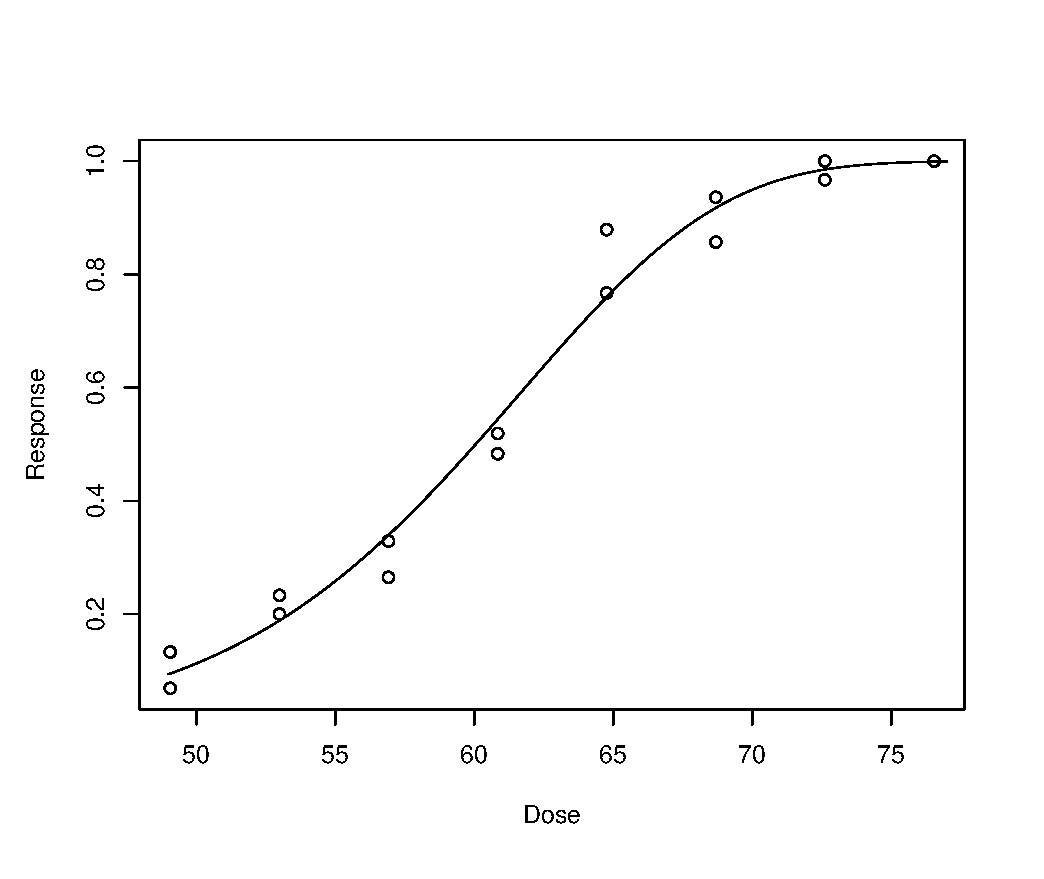
\includegraphics[width = 0.7\textwidth]{response.eps}
      \end{center}

      And the density of distribution of tolerance (dose) is 
      \begin{center}
      	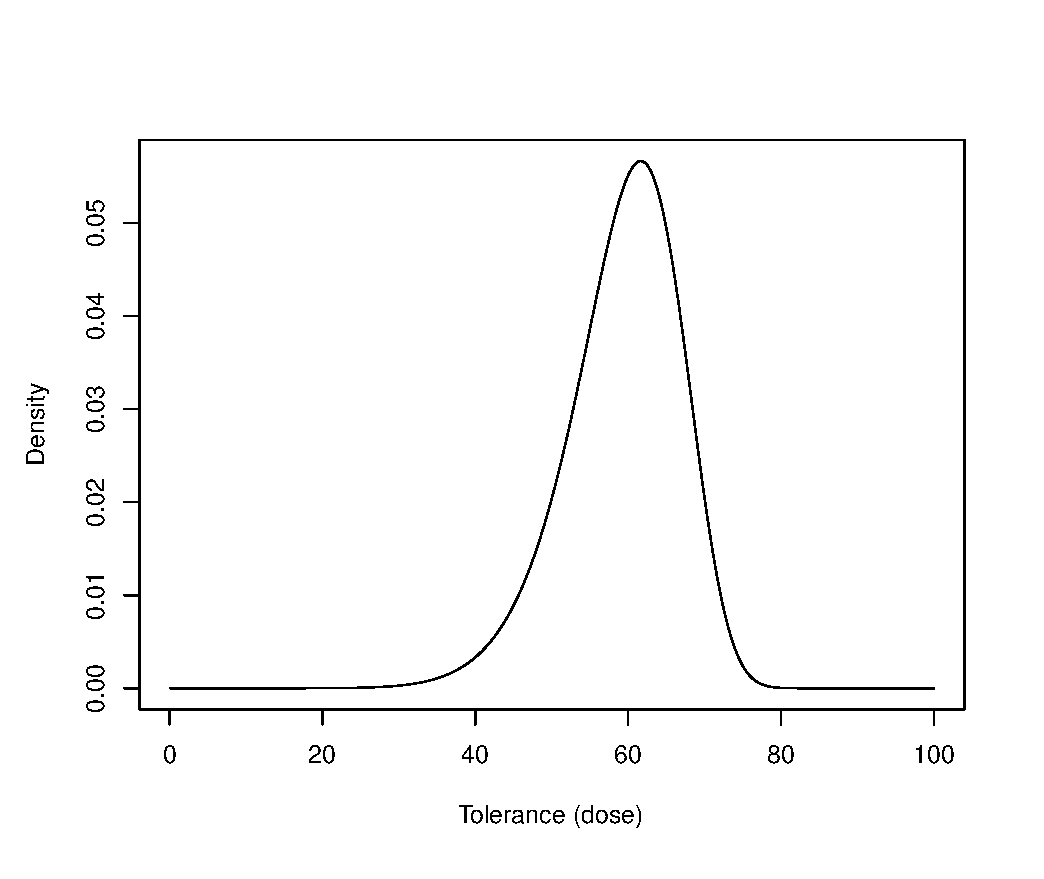
\includegraphics[width = 0.7\textwidth]{density.eps}
      \end{center}


      \item 
      We use generalized residuals to assess the fit of model. By probability integral transform, we transformed responses to $(0,1)$ by cdf of binomial distribution with parameters taken as estimated ones. Then we order the transformed responses and plot them against $\{1/(n+1), \ldots, n/(n+1)\}$, where $n$ is the total number of responses. The plot is shown below.
      \begin{center}
      	\includegraphics[width = 0.7\textwidth]{residual.eps}
      \end{center}

      From the plot, we can see the points fall in a line, but they are all above $y = x$ rather than fall evenly around it. So the fit of model is not so good based on the generalized residual plot. We need to find a better model.


      \item 
      The basic glm is fitted with function \verb|basicglm| from STAT 520. To fit glm with parameterized link, I wrote my own R code (specifically for this homework problem, not general one) for maximizing log likelihood using Fisher scoring algorithm. The code is written following algorithm steps on page 8 - 11 in the course notes.

 	\end{enumerate}






	
	
	
	\end{document}